\documentclass{standalone}
\usepackage{tikz}
\usetikzlibrary{patterns, positioning}


\begin{document}
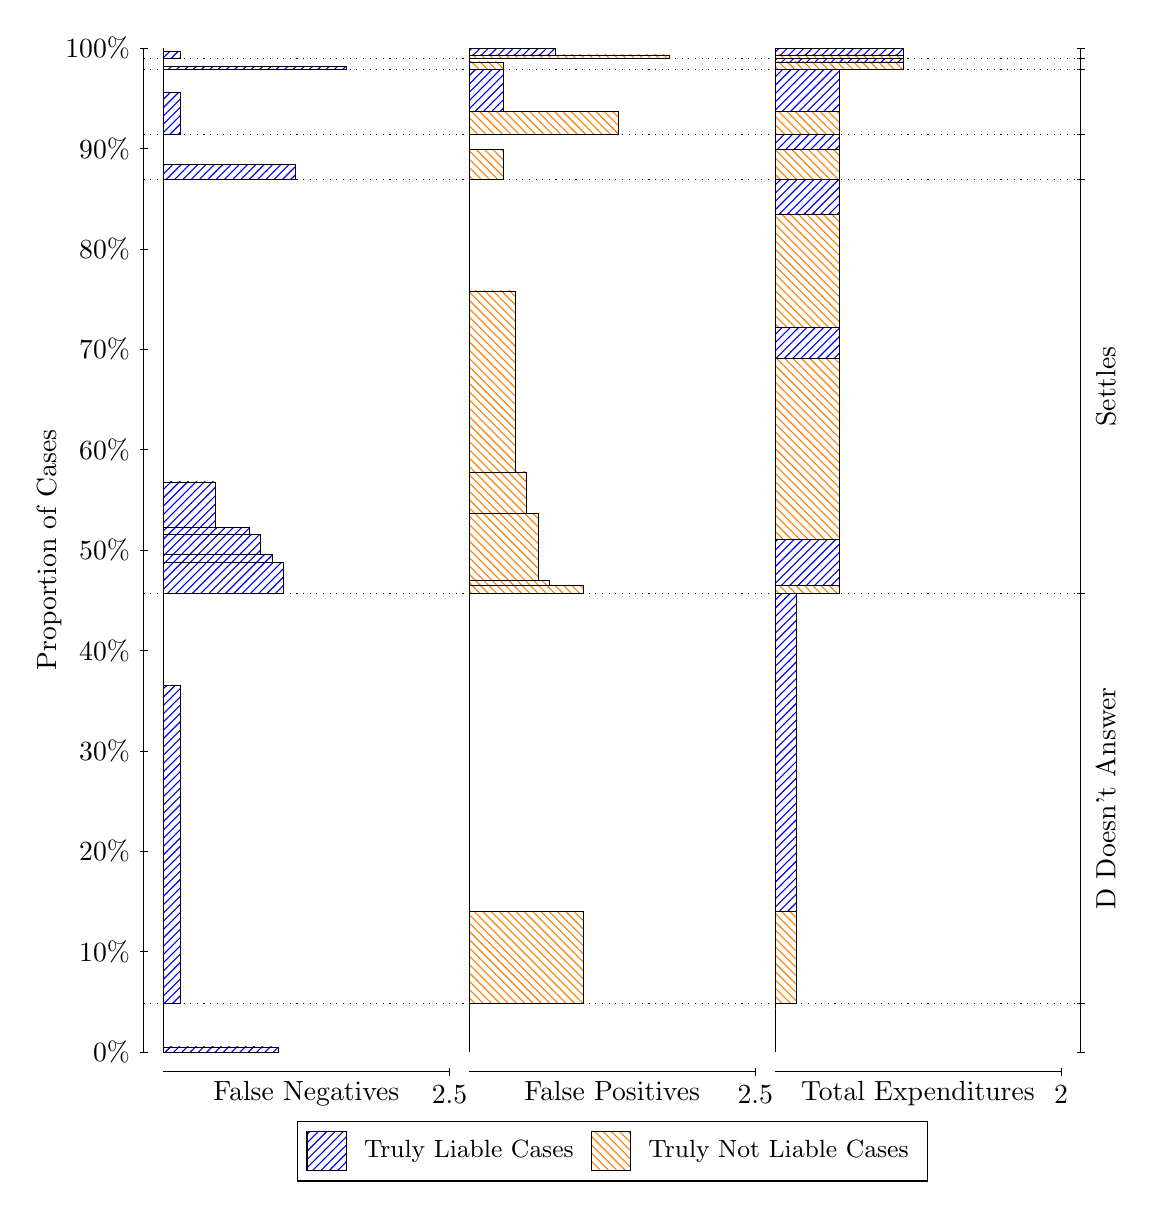
\begin{tikzpicture}
\draw[black, very thin] (1.5,1.75) -- (1.5,14.5);
\node[rotate=90, text=black, anchor=center] at (0.3, 8.125) {Proportion of Cases};
\draw[black, very thin] (1.45,1.75) -- (1.55,1.75);
\node[text=black, anchor=east] at (1.45, 1.75) {0\%};
\draw[black, very thin] (1.45,3.025) -- (1.55,3.025);
\node[text=black, anchor=east] at (1.45, 3.025) {10\%};
\draw[black, very thin] (1.45,4.3) -- (1.55,4.3);
\node[text=black, anchor=east] at (1.45, 4.3) {20\%};
\draw[black, very thin] (1.45,5.575) -- (1.55,5.575);
\node[text=black, anchor=east] at (1.45, 5.575) {30\%};
\draw[black, very thin] (1.45,6.85) -- (1.55,6.85);
\node[text=black, anchor=east] at (1.45, 6.85) {40\%};
\draw[black, very thin] (1.45,8.125) -- (1.55,8.125);
\node[text=black, anchor=east] at (1.45, 8.125) {50\%};
\draw[black, very thin] (1.45,9.4) -- (1.55,9.4);
\node[text=black, anchor=east] at (1.45, 9.4) {60\%};
\draw[black, very thin] (1.45,10.675) -- (1.55,10.675);
\node[text=black, anchor=east] at (1.45, 10.675) {70\%};
\draw[black, very thin] (1.45,11.95) -- (1.55,11.95);
\node[text=black, anchor=east] at (1.45, 11.95) {80\%};
\draw[black, very thin] (1.45,13.225) -- (1.55,13.225);
\node[text=black, anchor=east] at (1.45, 13.225) {90\%};
\draw[black, very thin] (1.45,14.5) -- (1.55,14.5);
\node[text=black, anchor=east] at (1.45, 14.5) {100\%};

\draw[black, very thin] (13.4,1.75) -- (13.4,14.5);
\draw[black, very thin] (13.35,1.75) -- (13.45,1.75);
\node[anchor=west] at (13.35, 1.75) {};
\draw[black, very thin] (13.35,2.3644) -- (13.45,2.3644);
\node[anchor=west] at (13.35, 2.3644) {};
\draw[black, very thin] (13.35,7.5731) -- (13.45,7.5731);
\node[anchor=west] at (13.35, 7.5731) {};
\draw[black, very thin] (13.35,12.833) -- (13.45,12.833);
\node[anchor=west] at (13.35, 12.833) {};
\draw[black, very thin] (13.35,13.407) -- (13.45,13.407);
\node[anchor=west] at (13.35, 13.407) {};
\draw[black, very thin] (13.35,14.226) -- (13.45,14.226);
\node[anchor=west] at (13.35, 14.226) {};
\draw[black, very thin] (13.35,14.367) -- (13.45,14.367);
\node[anchor=west] at (13.35, 14.367) {};
\draw[black, very thin] (13.35,14.5) -- (13.45,14.5);
\node[anchor=west] at (13.35, 14.5) {};

\draw[black, very thin, pattern color=blue, pattern=north east lines] (1.75,1.75) rectangle (3.2033,1.8146);
\draw[black, very thin, pattern color=orange, pattern=north west lines] (1.75,1.8146) rectangle (1.75,2.3644);
\draw[black, very thin, pattern color=blue, pattern=north east lines] (1.75,2.3644) rectangle (1.968,6.4046);
\draw[black, very thin, pattern color=orange, pattern=north west lines] (1.75,6.4046) rectangle (1.75,7.5731);
\draw[black, very thin, pattern color=blue, pattern=north east lines] (1.75,7.5731) rectangle (3.276,7.9703);
\draw[black, very thin, pattern color=blue, pattern=north east lines] (1.75,7.9703) rectangle (3.1307,8.0719);
\draw[black, very thin, pattern color=blue, pattern=north east lines] (1.75,8.0719) rectangle (2.9853,8.3257);
\draw[black, very thin, pattern color=blue, pattern=north east lines] (1.75,8.3257) rectangle (2.84,8.4082);
\draw[black, very thin, pattern color=blue, pattern=north east lines] (1.75,8.4082) rectangle (2.404,8.9907);
\draw[black, very thin, pattern color=orange, pattern=north west lines] (1.75,8.9907) rectangle (1.75,12.833);
\draw[black, very thin, pattern color=blue, pattern=north east lines] (1.75,12.833) rectangle (3.4213,13.026);
\draw[black, very thin, pattern color=orange, pattern=north west lines] (1.75,13.026) rectangle (1.75,13.407);
\draw[black, very thin, pattern color=blue, pattern=north east lines] (1.75,13.407) rectangle (1.968,13.933);
\draw[black, very thin, pattern color=orange, pattern=north west lines] (1.75,13.933) rectangle (1.75,14.226);
\draw[black, very thin, pattern color=blue, pattern=north east lines] (1.75,14.226) rectangle (4.0753,14.271);
\draw[black, very thin, pattern color=orange, pattern=north west lines] (1.75,14.271) rectangle (1.75,14.367);
\draw[black, very thin, pattern color=blue, pattern=north east lines] (1.75,14.367) rectangle (1.968,14.456);
\draw[black, very thin, pattern color=orange, pattern=north west lines] (1.75,14.456) rectangle (1.75,14.5);
\draw[black, very thin, pattern color=orange, pattern=north west lines] (5.6333,1.75) rectangle (5.6333,2.2998);
\draw[black, very thin, pattern color=blue, pattern=north east lines] (5.6333,2.2998) rectangle (5.6333,2.3644);
\draw[black, very thin, pattern color=orange, pattern=north west lines] (5.6333,2.3644) rectangle (7.0867,3.5329);
\draw[black, very thin, pattern color=blue, pattern=north east lines] (5.6333,3.5329) rectangle (5.6333,7.5731);
\draw[black, very thin, pattern color=orange, pattern=north west lines] (5.6333,7.5731) rectangle (7.0867,7.6775);
\draw[black, very thin, pattern color=orange, pattern=north west lines] (5.6333,7.6775) rectangle (6.6507,7.744);
\draw[black, very thin, pattern color=orange, pattern=north west lines] (5.6333,7.744) rectangle (6.5053,8.5892);
\draw[black, very thin, pattern color=orange, pattern=north west lines] (5.6333,8.5892) rectangle (6.36,9.1157);
\draw[black, very thin, pattern color=orange, pattern=north west lines] (5.6333,9.1157) rectangle (6.2147,11.415);
\draw[black, very thin, pattern color=blue, pattern=north east lines] (5.6333,11.415) rectangle (5.6333,12.833);
\draw[black, very thin, pattern color=orange, pattern=north west lines] (5.6333,12.833) rectangle (6.0693,13.213);
\draw[black, very thin, pattern color=blue, pattern=north east lines] (5.6333,13.213) rectangle (5.6333,13.407);
\draw[black, very thin, pattern color=orange, pattern=north west lines] (5.6333,13.407) rectangle (7.5227,13.7);
\draw[black, very thin, pattern color=blue, pattern=north east lines] (5.6333,13.7) rectangle (6.0693,14.226);
\draw[black, very thin, pattern color=orange, pattern=north west lines] (5.6333,14.226) rectangle (6.0693,14.323);
\draw[black, very thin, pattern color=blue, pattern=north east lines] (5.6333,14.323) rectangle (5.6333,14.367);
\draw[black, very thin, pattern color=orange, pattern=north west lines] (5.6333,14.367) rectangle (8.1767,14.412);
\draw[black, very thin, pattern color=blue, pattern=north east lines] (5.6333,14.412) rectangle (6.7233,14.5);
\draw[black, very thin, pattern color=orange, pattern=north west lines] (9.5167,1.75) rectangle (9.5167,2.2998);
\draw[black, very thin, pattern color=blue, pattern=north east lines] (9.5167,2.2998) rectangle (9.5167,2.3644);
\draw[black, very thin, pattern color=orange, pattern=north west lines] (9.5167,2.3644) rectangle (9.7892,3.5329);
\draw[black, very thin, pattern color=blue, pattern=north east lines] (9.5167,3.5329) rectangle (9.7892,7.5731);
\draw[black, very thin, pattern color=orange, pattern=north west lines] (9.5167,7.5731) rectangle (10.334,7.6775);
\draw[black, very thin, pattern color=blue, pattern=north east lines] (9.5167,7.6775) rectangle (10.334,8.26);
\draw[black, very thin, pattern color=orange, pattern=north west lines] (9.5167,8.26) rectangle (10.334,10.559);
\draw[black, very thin, pattern color=blue, pattern=north east lines] (9.5167,10.559) rectangle (10.334,10.957);
\draw[black, very thin, pattern color=orange, pattern=north west lines] (9.5167,10.957) rectangle (10.334,12.395);
\draw[black, very thin, pattern color=blue, pattern=north east lines] (9.5167,12.395) rectangle (10.334,12.833);
\draw[black, very thin, pattern color=orange, pattern=north west lines] (9.5167,12.833) rectangle (10.334,13.213);
\draw[black, very thin, pattern color=blue, pattern=north east lines] (9.5167,13.213) rectangle (10.334,13.407);
\draw[black, very thin, pattern color=orange, pattern=north west lines] (9.5167,13.407) rectangle (10.334,13.7);
\draw[black, very thin, pattern color=blue, pattern=north east lines] (9.5167,13.7) rectangle (10.334,14.226);
\draw[black, very thin, pattern color=orange, pattern=north west lines] (9.5167,14.226) rectangle (11.152,14.323);
\draw[black, very thin, pattern color=blue, pattern=north east lines] (9.5167,14.323) rectangle (11.152,14.367);
\draw[black, very thin, pattern color=orange, pattern=north west lines] (9.5167,14.367) rectangle (11.152,14.412);
\draw[black, very thin, pattern color=blue, pattern=north east lines] (9.5167,14.412) rectangle (11.152,14.5);
\draw[black, dotted] (1.5,2.3644) -- (13.4,2.3644);
\draw[black, dotted] (1.5,7.5731) -- (13.4,7.5731);
\draw[black, dotted] (1.5,12.833) -- (13.4,12.833);
\draw[black, dotted] (1.5,13.407) -- (13.4,13.407);
\draw[black, dotted] (1.5,14.226) -- (13.4,14.226);
\draw[black, dotted] (1.5,14.367) -- (13.4,14.367);
\draw[black, very thin] (1.75,1.5) -- (5.3833,1.5);
\node[text=black, anchor=north] at (3.5667, 1.5) {False Negatives};
\draw[black, very thin] (5.3833,1.45) -- (5.3833,1.55);
\node[text=black, anchor=north] at (5.3833, 1.45) {2.5};

\draw[black, very thin] (5.6333,1.5) -- (9.2667,1.5);
\node[text=black, anchor=north] at (7.45, 1.5) {False Positives};
\draw[black, very thin] (9.2667,1.45) -- (9.2667,1.55);
\node[text=black, anchor=north] at (9.2667, 1.45) {2.5};

\draw[black, very thin] (9.5167,1.5) -- (13.15,1.5);
\node[text=black, anchor=north] at (11.333, 1.5) {Total Expenditures};
\draw[black, very thin] (13.15,1.45) -- (13.15,1.55);
\node[text=black, anchor=north] at (13.15, 1.45) {2};


\node[text=black, centered, rotate=90] at (13.72, 4.9688) {D Doesn't Answer};
\node[text=black, centered, rotate=90] at (13.72, 10.203) {Settles};





\draw (7.449999999999999,1.5) node[draw=none] (baseCoordinate) {};
\begin{scope}[align=center]
        \matrix[scale=0.5, draw=black, below=0.5cm of baseCoordinate, nodes={draw}, column sep=0.1cm]{
            \node[rectangle, draw, minimum width=0.5cm, minimum height=0.5cm, pattern color=blue, pattern=north east lines] {}; &
            \node[draw=none, font=\small, text=black] (B) {Truly Liable Cases}; &
            \node[rectangle, draw, minimum width=0.5cm, minimum height=0.5cm, pattern color=orange, pattern=north west lines] {}; &
            \node[draw=none, font=\small, text=black] (B) {Truly Not Liable Cases}; \\
            };
\end{scope}

\end{tikzpicture}
\end{document}